\documentclass{article}
\usepackage{tikz}
\usetikzlibrary{arrows,decorations.pathmorphing,backgrounds,positioning,fit,petri}

\begin{document}

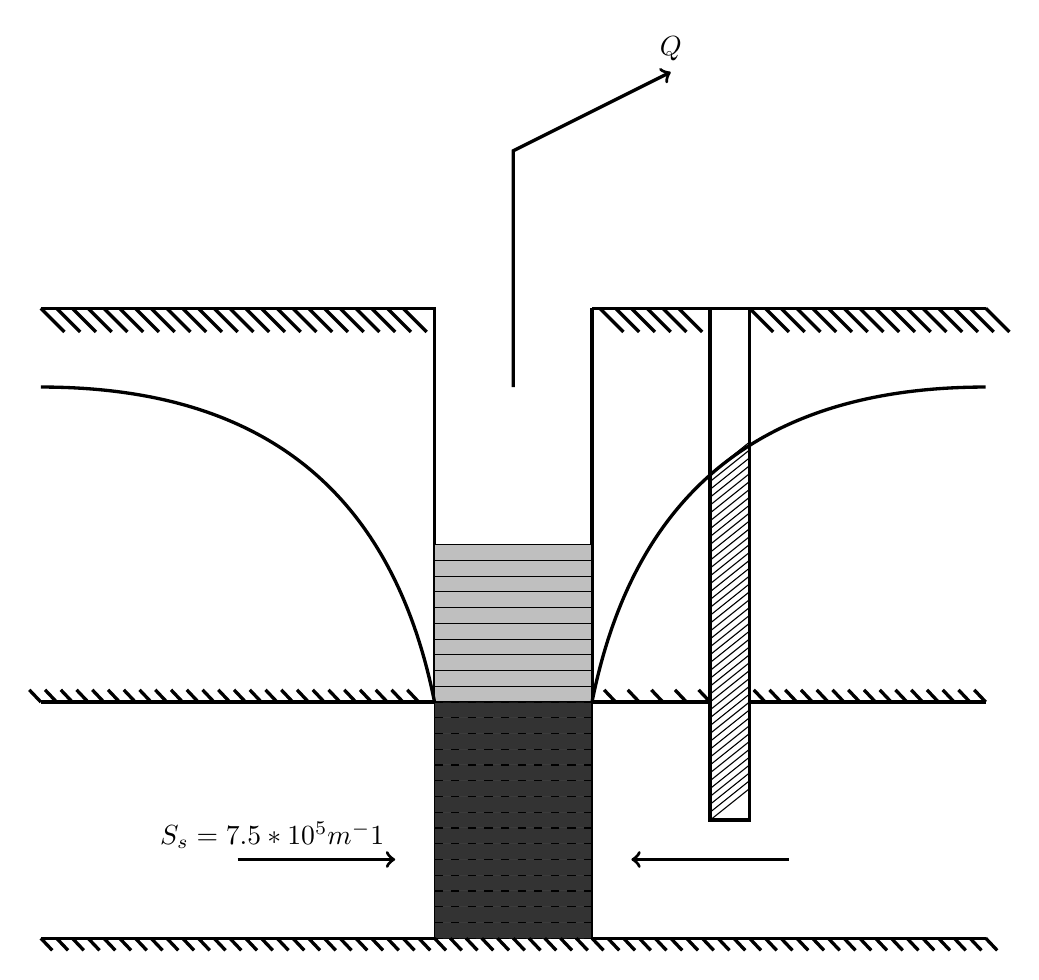
\begin{tikzpicture}
	%Draws the top of the subsurface i.e. above the confined aquifer
	\draw (-6,0) -- (-1,0) -- (-1,-5) -- (-6,-5)   [very thick];
	\draw (6,0) -- (3,0) [very thick];
	\draw ( 2.5,0) --(1,0) [very thick];
	\draw (1,0)--(1,-5) [very thick];
	\draw (1,-5)--(2.5,-5) [very thick]; 
	\draw (3,-5)--(6,-5)  [very thick];

	%Draws the bottom of the confined aquifer
	\draw (-1,-8) -- (-6,-8) [very thick];
	\draw  (1,-8) -- (6,-8)[very thick];

	\foreach \x in {-6,-5.8,...,-1.4}
		\draw [very thick](\x,0) -- (\x+0.3,-.3);

	\foreach \x in {6,5.8,...,3,2.1,1.9,...,1.0}
		\draw[very thick] (\x,0) -- (\x+0.3,-.3);

	%Draws the area of the well directly above the confined aquifer
	\filldraw[fill=gray!50] (-1,-3) rectangle (1,-5);
	\foreach \y in {-5,-4.8,...,-3}
		\draw[very thin] (-1,\y) -- (1,\y);

	\foreach \x in {-6,-5.8,...,-1.2}
		\draw [very thick] (\x, -5,0) -- (-.3+\x,-5,-0.4pt);

	\foreach \x in {6,5.8,...,3.2,2.5,2.2,...,1.2}
		\draw[very thick] (\x,-5,0) -- (-.3+\x,-5,-.4pt);
	%Draws the well directly in the confined aquifer
	\filldraw[fill=black!80] (-1,-5) rectangle (1,-8);
	
	\foreach \y in {-8,-7.8,...,-5}	
		\draw[style=dashed, fill=gray] 
			(-1,\y) -- (1,\y);

	\foreach \x in {-6,-5.8,...,6}
		\draw[very thick] (\x,-8,0) -- (\x+.3,-8,.4pt);
       
	%Draws the piezometer
	\draw [very thick](2.5,-6.5) rectangle (3,0);

	\foreach \y in {-6.5,-6.4,...,-2}
		\draw (2.5,\y)--(3,\y+.4);

	%Draws the draw down curve experienced in the confined aquifer
	\draw[very thick] (-1,-5) .. controls (-1.5,-2.5) and (-3,-1) .. (-6,-1);
	\draw[very thick] (1,-5) .. controls (1.5,-2.5) and (3,-1) .. (6,-1);

	%Attributes of the confined aquifer (arrow and fill pattern)
	\draw[->][very thick] (-3.5,-7)--(-1.5,-7) node[anchor=south east] {$S_s=7.5 * 10^5 m^-1$} ;
	\draw[->][very thick] (3.5,-7.0)--(1.5,-7);

	%Define Parameters
	\draw[->][very thick] (0,-1) -- (0,2)--(2,3)[very thick] node[anchor=south] {$Q$};
	

	
	
	
	


	

	
\end{tikzpicture}
\end{document}